\section{Versuchsdurchführung}
\label{section:Versuchsdurchführung}
Der Versuch wurde am 23.06.2023 zwischen 11:30 Uhr und 13:00 Uhr durchgeführt. 
Die Wetterbedingungen am besagten Tag waren nahezu optimal für diesen Versuch. 
Dies zeichnete sich dadurch aus, dass der Himmel vollständig bedeckt war, was die 
Annahme zulässt, dass kaum direkte Bestrahlung Einfluss auf die Ergebnisse nehmen würde. 
Begonnen wurde der Versuch damit, dass der Raum von allem unnötigem Mobiliar befreit wurde.
Anschließend wurde der Raum vollständig vermessen. Fokus lag hierbei auf der Position 
der Lampen, sowie Fenster.\\
Das Ergebnis dieser Messungen ist der in \autoref{fig:grundriss} zu sehende Grundriss.
Aus dem entstandenen Grundriss ist zusätzlich ein einfaches dreidimensionales Modell erstellt wurden,
dieses ist in \autoref{fig:3D-Model} dargestellt.

\begin{figure}[H]
        \centering
        \begin{minipage}[b]{0.4\textwidth}
            \centering
            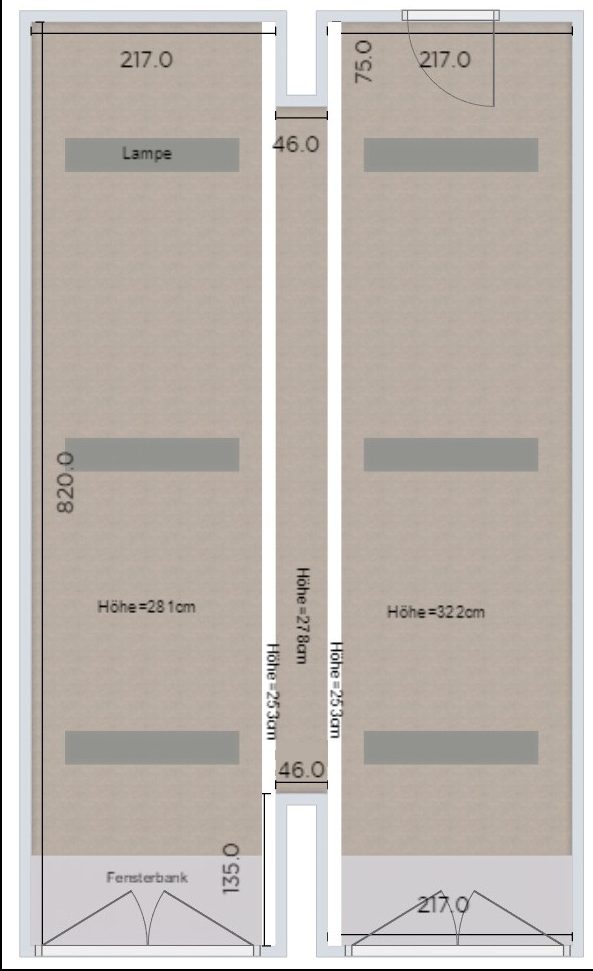
\includegraphics[width=\textwidth]{Abbildungen/Grundriss.jpg}
            \caption{Grundriss: Raum G319}
            \label{fig:grundriss}    
        \end{minipage}
        \hfill
        \begin{minipage}[b]{0.49\textwidth}
            \centering
            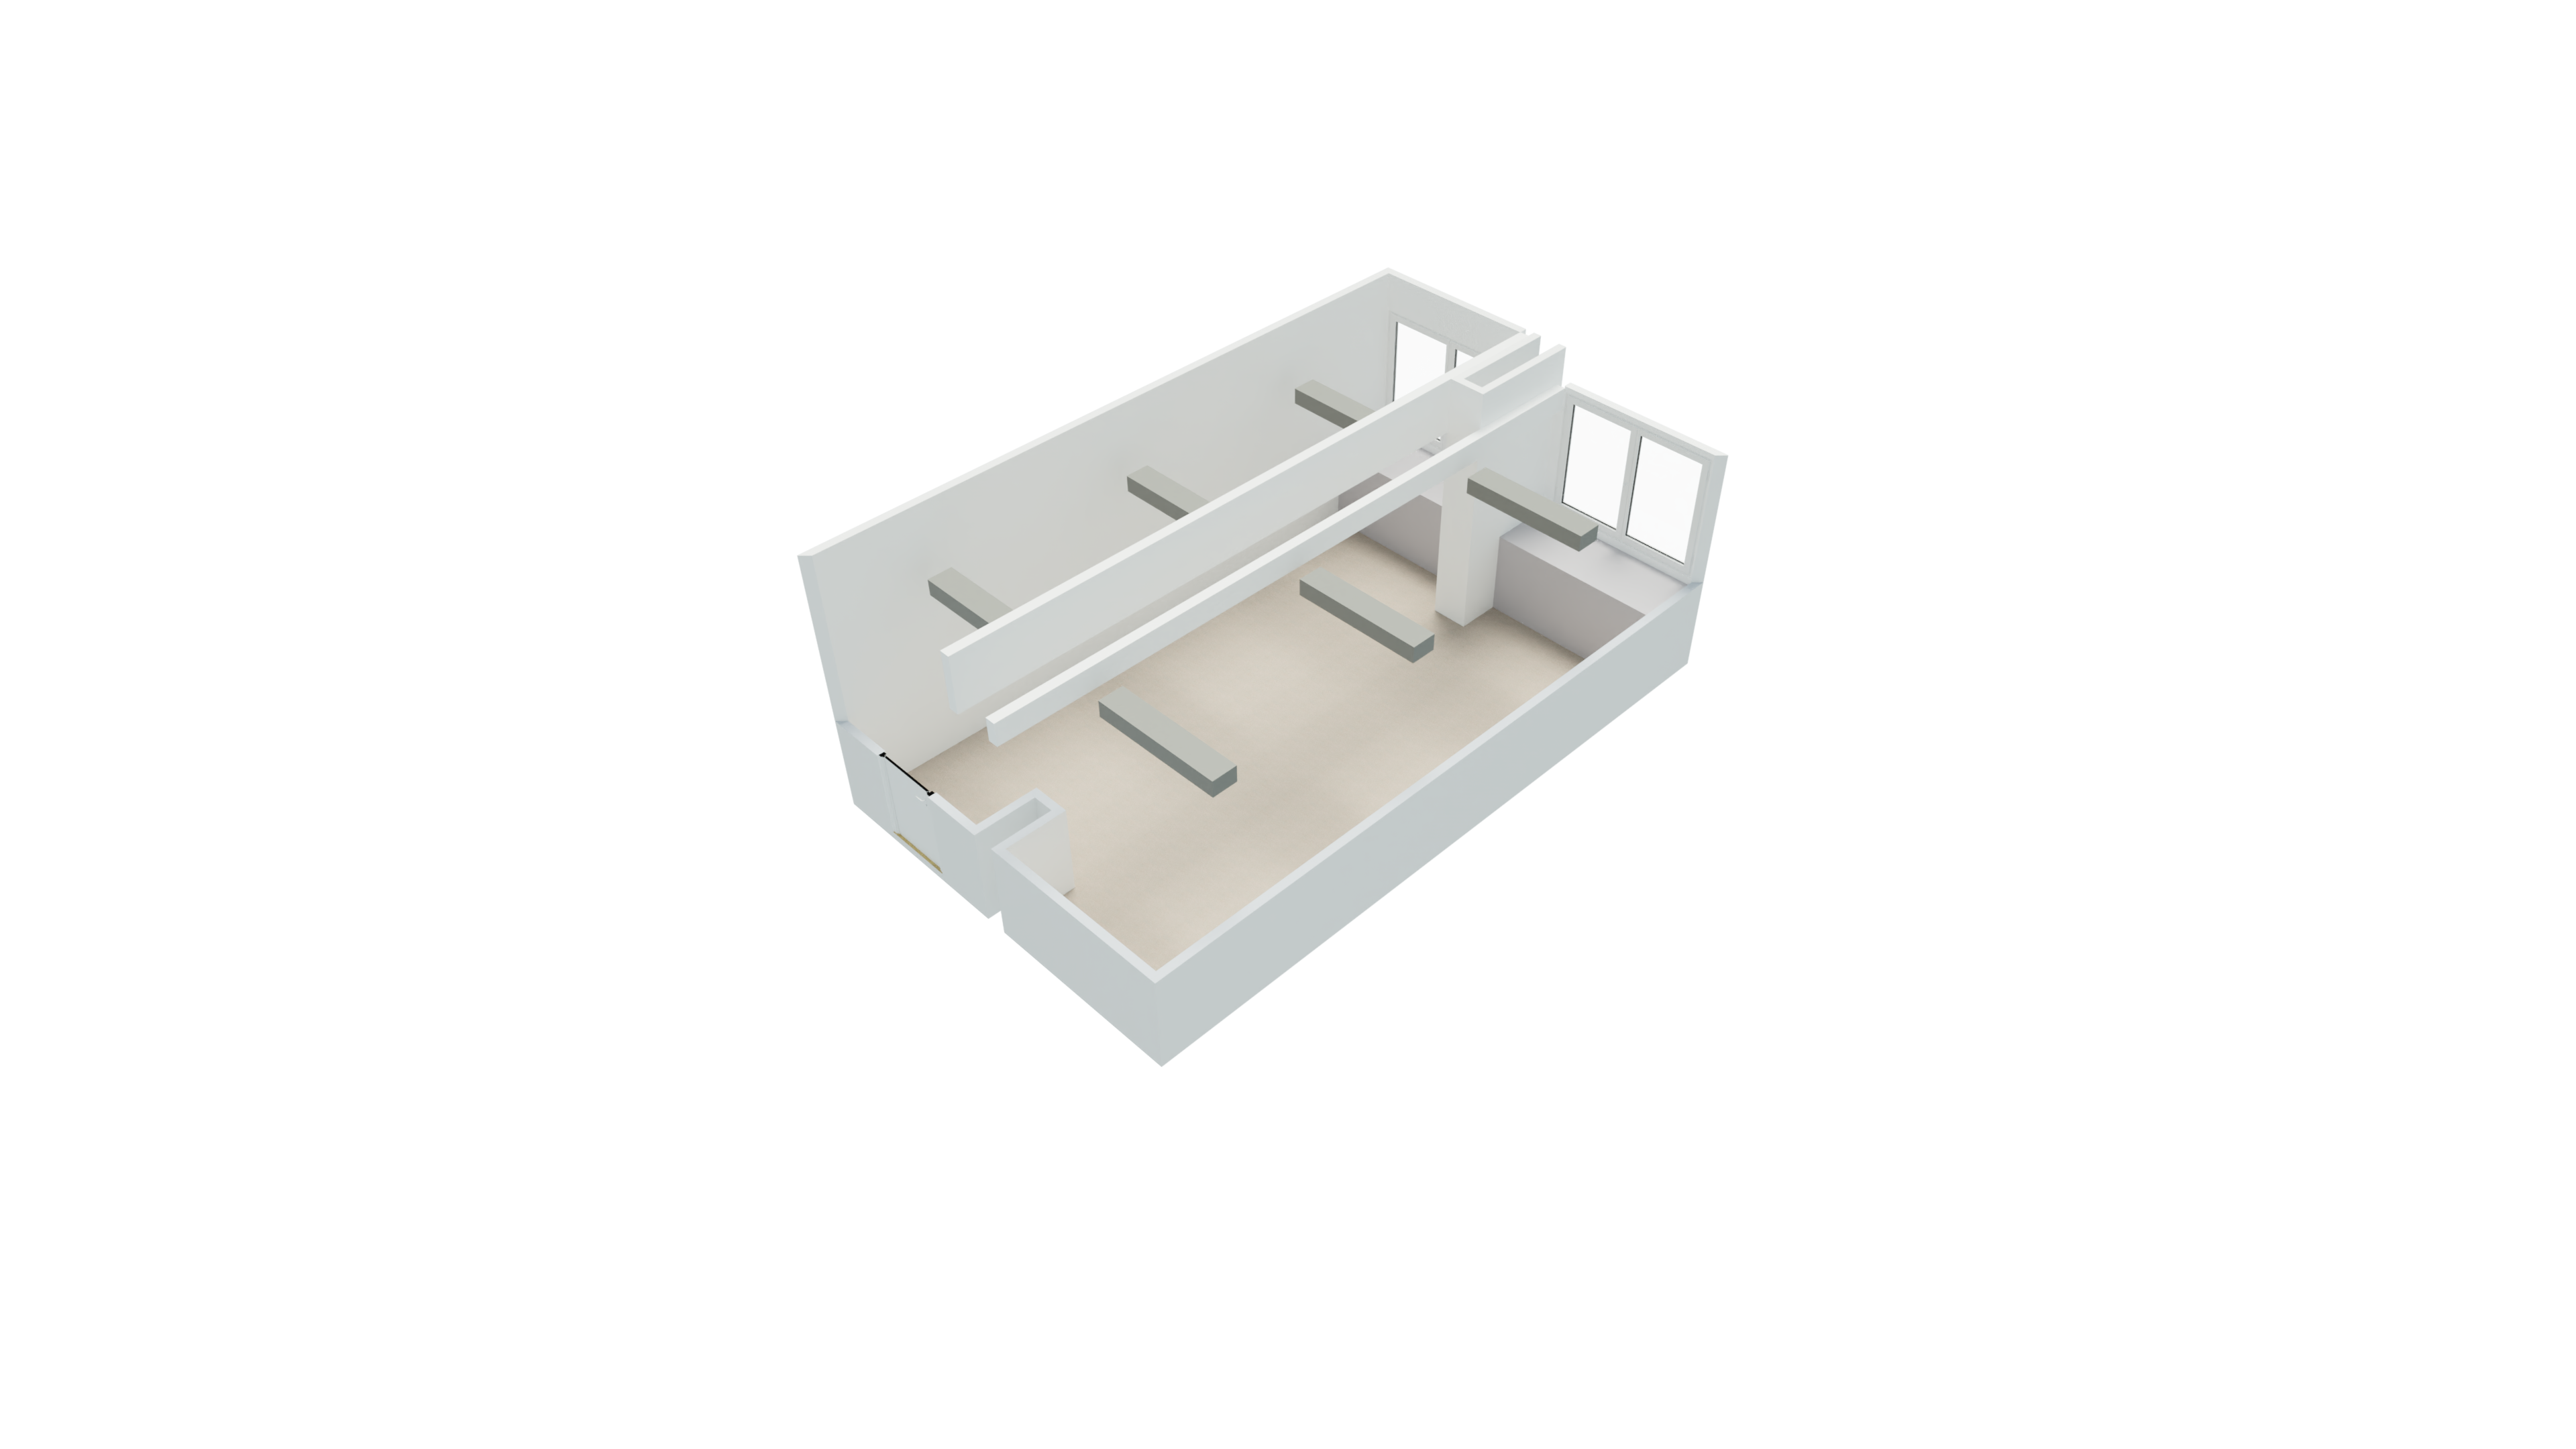
\includegraphics[scale=0.25]{Abbildungen/3D-Model.png}
            \caption{3D-Model: Raum G319}
            \label{fig:3D-Model}    
        \end{minipage}
\end{figure}

Sobald das Vermessen des Raumes abgeschlossen war, wurde die Versuchsgruppe
aufgeteilt. Ein Teil der Gruppe blieb im Raum und führte dort die Messungen durch
während der andere Teil die Messungen mit dem externen Luxmeter auf dem Dach durchführte. 
Um zu ermöglichen, dass die Messwerte an beiden Messstellen zeitgleich aufgenommen werden,
verständigte sich die Gruppe via Mobiltelefon.\\
Die Messwerte wurden sowohl von dem Laptop als auch von dem Luxmeter auf dem Dach
abfotografiert und für die anschließende Auswertung in einer Tabellenkalkulation zusammengetragen. 
Messwerte wurden an drei unterschiedlichen Positionen im Raum gemessen, hierbei wurde
das Messgerüst fortlaufend weiter von den Fenstern entfernt.
Für jede der drei Positionen wurden die folgenden drei Fälle betrachtet und mit jedem der 11 Sensoren ein Wert aufgenommen: 
\small
\begin{multicols}{3}
    \begin{itemize}
        \item Fenster geschlossen, Licht aus
        \item Fenster geöffnet, Licht aus
        \item Fenster geschlossen, Licht an
    \end{itemize}
\end{multicols}


